\documentclass{uninove-ppgi} %courier ou times

\begin{document}
\lstset{
    language=xml,
    tabsize=3,
    frame=shadowbox,
    rulesepcolor=\color{gray},
    xleftmargin=20pt,
    framexleftmargin=15pt,
    keywordstyle=\color{blue}\bf,
    commentstyle=\color{OliveGreen},
    stringstyle=\color{red},
    numbers=left,
    numberstyle=\tiny,
    numbersep=5pt,
    breaklines=true,
    showstringspaces=false,
    basicstyle=\footnotesize,
    emph={food,name,price},emphstyle={\color{magenta}}
}

% Posiciona o logo da Uni9 no topo
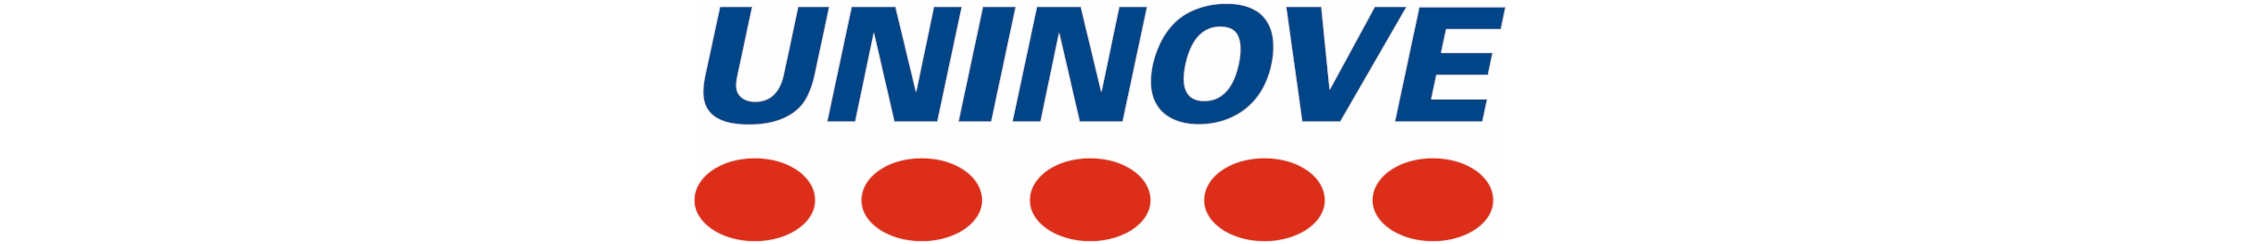
\includegraphics[height=1.5cm]{uninove-logo}

% parametros de capa e folha de rosto (é necessário configurar todos)
\Universidade{UNIVERSIDADE NOVE DE JULHO - UNINOVE}

% Os nomes deverão estar em ordem alfabética OBRIGATORIAMENTE
\Autor{618250080 - EDSON MELO DE SOUZA\\
    618250080 - EDSON MELO DE SOUZA\\
    618250080 - EDSON MELO DE SOUZA\\
    618250080 - EDSON MELO DE SOUZA\\
    618250080 - EDSON MELO DE SOUZA\\
    618250080 - EDSON MELO DE SOUZA\\
    618250080 - EDSON MELO DE SOUZA\\
    618250080 - EDSON MELO DE SOUZA\\
    618250080 - EDSON MELO DE SOUZA\\
    618250080 - EDSON MELO DE SOUZA}

\Titulo{TÍTULO DO TRABALHO}

% Inserir o nome do projeto no formato que está abaixo (Olhe o nome da disciplina na central do aluno)
\Tipoprojeto{PROJETO EM SISTEMAS INTERATIVOS}

% Informe qual o curso: Bacharel ou Tecnólogo + curso
\Curso{Bacharel em Ciência da Computação}

% NÃO ALTERAR
\Orientador{Edson Melo de Souza, Dr.}

% Inserir o ano correspondente
\Ano{202X}

% gera a capa automaticamente
\capa

% gera folha de rosto automaticamente
\folharosto

% ##################### Início dos elementos pré-textuais ############################

% Resumo (Obrigatório)
% !TEX root = ..\main.tex

\PalavrasChave{Palavra 1, Palavra 2, Palavra 3, Palavra 4, Palavra 5, Palavra 6.}
\centeredchapterstyle
\begin{resumo}
    \noindent\textbf{Contexto}: Nisi mollit anim consequat deserunt tempor laboris fugiat sit do. Pariatur duis est incididunt deserunt pariatur quis sint. Consectetur aliqua reprehenderit laborum aute id dolor fugiat. In consequat pariatur officia dolor esse pariatur sit reprehenderit. Duis nostrud proident occaecat non adipisicing officia sit sunt aute. Nulla eiusmod labore elit velit. Labore fugiat dolor sint irure Lorem irure est voluptate dolor magna commodo. \textbf{Objetivo}: Consequat velit incididunt laborum sit reprehenderit ea ex cillum ut ut incididunt veniam veniam id. \textbf{Método}: Deserunt labore labore reprehenderit fugiat dolor Lorem enim consequat ea. Reprehenderit officia id eiusmod voluptate dolor excepteur. Ut adipisicing occaecat laboris minim laborum dolore tempor. Veniam aliqua ad exercitation aute Lorem veniam laborum voluptate anim sunt enim. \textbf{Resultados}: Deserunt labore labore reprehenderit fugiat dolor Lorem enim consequat ea. Reprehenderit officia id eiusmod voluptate dolor excepteur. Ut adipisicing occaecat laboris minim laborum dolore tempor. Veniam aliqua ad exercitation aute Lorem veniam laborum voluptate anim sunt enim. \textbf{Conclusão}: Deserunt labore labore reprehenderit fugiat dolor Lorem enim consequat ea. Reprehenderit officia id eiusmod voluptate dolor excepteur. Ut adipisicing occaecat laboris minim laborum dolore tempor. Veniam aliqua ad exercitation aute Lorem veniam laborum voluptate anim sunt enim.
\end{resumo}

% Abstract (Obrigatório) - resumo em inglês
% !TEX root = ..\main.tex

\KeyWords{Keyword 1, Keyword 2, Keyword 3, Keyword 4, Keyword 5, Keyword 6.}
\centeredchapterstyle
\begin{abstract}
    \noindent\textbf{Contextualization}: Nisi mollit anim consequat deserunt tempor laboris fugiat sit do. Pariatur duis est incididunt deserunt pariatur quis sint. Consectetur aliqua reprehenderit laborum aute id dolor fugiat. In consequat pariatur officia dolor esse pariatur sit reprehenderit. Duis nostrud proident occaecat non adipisicing officia sit sunt aute. Nulla eiusmod labore elit velit. Labore fugiat dolor sint irure Lorem irure est voluptate dolor magna commodo. \textbf{Objetive}: Consequat velit incididunt laborum sit reprehenderit ea ex cillum ut ut incididunt veniam veniam id. \textbf{Method}: Deserunt labore labore reprehenderit fugiat dolor Lorem enim consequat ea. Reprehenderit officia id eiusmod voluptate dolor excepteur. Ut adipisicing occaecat laboris minim laborum dolore tempor. Veniam aliqua ad exercitation aute Lorem veniam laborum voluptate anim sunt enim. \textbf{Results}: Deserunt labore labore reprehenderit fugiat dolor Lorem enim consequat ea. Reprehenderit officia id eiusmod voluptate dolor excepteur. Ut adipisicing occaecat laboris minim laborum dolore tempor. Veniam aliqua ad exercitation aute Lorem veniam laborum voluptate anim sunt enim. \textbf{Conclusion}: Deserunt labore labore reprehenderit fugiat dolor Lorem enim consequat ea. Reprehenderit officia id eiusmod voluptate dolor excepteur. Ut adipisicing occaecat laboris minim laborum dolore tempor. Veniam aliqua ad exercitation aute Lorem veniam laborum voluptate anim sunt enim.
\end{abstract}


% Sumário (Obrigatório)
\begingroup
\makeatletter \let\ps@plain\ps@empty \makeatother
\tableofcontents
\endgroup
\thispagestyle{empty}

% Lista de figuras
\renewcommand*\listfigurename{Lista de Ilustrações}
\listoffigures
\thispagestyle{empty}

% Lista de tabelas
\listoftables
\thispagestyle{empty}

% Lista de quadros
\listofquadros
\thispagestyle{empty}

% Lista de abreviaturas (Opcional)
\begin{listaabreviaturas}%
    MM & Morfologia matemática \\
    CC & Componente conexo \\
    EE & Elemento estruturante
\end{listaabreviaturas}

% ############### Fim dos elementos pré-textuais ######################

\regularchapterstyle

% ############### Início dos Capítulos (Obrigatório ) #################

% Introdução
\chapter{Introdução}
\label{ch:introducao}
\begin{resumocapitulo}
	Este resumo pode ser utilizado para melhorar a comunicação com o leitor. As seções e subseções são configuradas de acordo com a normas ABNT (2020) adotada pela Universidade Nove de Julho - Uninove (tamanho da fonte, espaçamento...). As numerações de página estão alinhadas a direita no cabeçalho. Neste capítulo são mostrados exemplos para utilização de comandos de \textbf{citação} (\textit{arquivo refs.bib}), \textbf{tabelas}, \textbf{quadros}, \textbf{equações} e \textbf{algoritmos}. Para ter acesso a documentação diretamente na biblioteca da Uninove, \href{http://docs.uninove.br/arte/pdfs/Manual_de_Trabalhos_Academicos_ABNT_UNINOVE.pdf}{clique aqui.}
\end{resumocapitulo}

\section{Citações diretas e indiretas}
\label{sec:citacoes}
\subsection{Citação Direta}
\label{subsec:citacao_direta}
O comando \texttt{$\backslash$citeonline\{Referencia-refs.bib\}} gera o seguinte resultado:

Segundo \citeonline{mitchell1997machine}, aprendizagem de máquina ``[...] é como um programa de computador aprende pela experiência \textit{E}, com respeito a algum tipo de tarefa \textit{T} e performance \textit{P}, se sua performance \textit{P} nas tarefas em \textit{T}, na forma medida por \textit{P}, melhoram com a experiência''.

\subsection{Citação Indireta}
\label{subsec:citacao_indireta}
O comando \texttt{$\backslash$cite\{Referencia-refs.bib\}} gera o seguinte resultado:

O SCImago é um portal que fornece indicadores de produções científicas contidas no banco de dados do Scopus \cite{Villasenor-Almaraz2019}, sobre os principais periódicos do mundo \cite{DUggento2016}.

\section{Montagem de Tabela}
\label{sec:tabela}
A seguir o exemplo de uma tabela, Tabela~\ref{tab:tab_identificador}. Para tabelas mais complexas acesse \textbf{Tables Generator} (\href{https://www.tablesgenerator.com/}{https://www.tablesgenerator.com}).
\begin{table}[!ht]
	\centering
	\caption{Descrição da tabela}
	\label{tab:tab_identificador}
	\begin{tabular*}{\columnwidth}{@{\extracolsep{\fill}}lrccc@{}}
		\toprule[1pt]{}\textbf{Desc. 1} & \textbf{Desc. 2} & \textbf{Desc. 4} & \textbf{Desc. 5} & \textbf{Desc. 6}\\\hline
		Item 1		& 901     	& 376  	& 4,738 & 21,317	\\
		Item 2		& 790		& 654  	& 5,913 & 45,540	\\
		Item 3 		& 333		& 215  	& 5,616 & 10,500	\\
		\bottomrule[1pt]
	\end{tabular*}
	\raggedright
	\amostra{2.024} \\% determina o tamanho de uma amostra
	\fontetabela{Autor} % alinha o nome do autor à esquerda
\end{table}

% \begin{landscape}
% 	\begin{table}[!ht]
% 		\small
% 		\centering
% 		\begin{tabular}{llllllllllll}
% 			\hline
% 			\\
% 			\multicolumn{12}{l}{\textbf{Total trade by country and by year (in US\$)}}    \\
% 			\hline \hline
% 			\\
% 			 & 2003 & 2004 & 2005 & 2006 & 2007 & 2008 & 2009 & 2010 & 2011 & 2012 & 2013 \\
% 			...
% 		\end{tabular}
% 		\caption{Trade volume evolution Costa Rica - EFTA}
% 		\label{tbl:tradeevo-costa-efta}
% 	\end{table}
% \end{landscape}


\begin{landscape}
	\begin{table}[!ht]
		\small
		\centering
		\caption{Formatação no modo paisagem para textos grandes.}
		\label{tab:loadings}
		\begin{tabular*}{\columnwidth}{@{\extracolsep{\fill}}lccc@{}}
			\toprule[1pt]{}\textbf{Categories}      & \textbf{Factor 1} & \textbf{Factor 2} & \textbf{Communality}
			\\\hline
			Study Concept           & 0.645		& 0.324   & 0.52	\\
			Study Supervision		& 0.628		& 0.116   & 0.41	\\
			Funding and/or Support  & 0.484		& 0.144   & 0.24	\\
			Critical Revision   	& 0.441		& 0.238   & 0.25	\\
			Study Concept           & 0.645		& 0.324   & 0.52	\\
			Study Supervision		& 0.628		& 0.116   & 0.41	\\
			Funding and/or Support  & 0.484		& 0.144   & 0.24	\\
			Critical Revision   	& 0.441		& 0.238   & 0.25	\\
			Statistical Analysis 	& 0.107		& 0.724  & 0.54		\\
			Original Draft			& 0.338		& 0.525  & 0.38		\\
			Data Collection			& 0.245   	& 0.275  & 0.14		\\
			Statistical Analysis 	& 0.107		& 0.724  & 0.54		\\
			Original Draft			& 0.338		& 0.525  & 0.38		\\
			Data Collection			& 0.245   	& 0.275  & 0.14		\\
			\hline \\[-1.8ex]
			\textit{Cronbach's $\alpha$}	& \textit{0.656}     & \textit{0.550}  \\
			\bottomrule[1pt]
		\end{tabular*}
		\fonte{Autor}
	\end{table}
\end{landscape}

\section{Montagem de Quadro}
\label{sec:quadro}
Os quadros também podem ser posicionados no modo paisagem, conforme as configurações da tabela anterior. É importante destacar que um quadro não pode ser colocado em um parágrafo, mas sim em uma seção ou capítulo. A característica principal de uma Quadro em relação a uma Tabela, é que Quadros possuem texto, enquanto as Tabelas só contém números (excetos o cabeçalho).

\begin{quadros}[ht!]
	\caption{Descrição dos dados contidos no quadro.}
	\label{quad:contribuicoes_annals}
	\centering
	\begin{small}
		\def\arraystretch{1.1}
		\begin{tabular}{|p{1.0cm}|p{14.0cm}|}
			\hline
			\textbf{\#} & \textbf{Descrição} \\\hline
			1           & \textit{Linha 1}   \\\hline
			2           & \textit{Linha 2}   \\\hline
			3           & \textit{Linha 3}   \\\hline
			4           & \textit{Linha 4}   \\\hline
			5           & \textit{Linha 5}   \\\hline
		\end{tabular}
	\end{small}
	\fonte{\cite{Abbasi2011}}
\end{quadros}

\section{Montagem de Equação}
\label{sec:equacao}
\begin{definicao}{Média aritmética}
	Para uma amostra $ X=\{x_1,, x_2, \ldots,x_n\} $ de observações, onde $ n $ é o número de observações, se define a média aritmética da seguinte forma:
	\begin{equation}
		\mu(X)=\dfrac{1}{n}\sum\limits_{x \in X}x
	\end{equation}
\end{definicao}
\begin{proposicao}
	Se $ k $ é uma constante então multiplicar a média de uma amostra $ X $ é o mesmo de multiplicar cada elemento de $ X $ por $ k $, isto é, $ k \times \mu(X) = \dfrac{1}{n} \sum\limits_{x \in X}x\times k $.
\end{proposicao}
\begin{prova}
	Desenvolve-se a igualdade:
	\begin{align*}
		k \times \mu(X) & = \dfrac{1}{n} \sum\limits_{x \in X}xk                           \\
		                & \Longleftrightarrow  \dfrac{(x_1k,x_2k, \ldots, x_nk)}{n}        \\
		                & \Longleftrightarrow  \dfrac{nk \times (x_1,x_2, \ldots, x_n)}{n} \\
		                & \Longleftrightarrow   k \times \dfrac{(x_1,x_2, \ldots, x_n)}{n} \\
		                & \Longleftrightarrow   k \times \mu(X) \numberequation{1}
	\end{align*}
\end{prova}
Assim, concluí-se que $ k \times \mu(X) = \dfrac{1}{n} \sum\limits_{x \in X}x\times k $.

\section{Montagem de Algoritmo}
\label{sec:algortimo}
Apresentação do Algoritmo~\ref{algorithm:algoritmo_descricao}.
\begin{algorithm}
	\SetInd{0.5cm}{0.1cm}
	\Entrada{$Artigos$}
	\Saida{$Dataset$}
	\SetAlgoLined

	$ Dataset \leftarrow \emptyset $ \\
	\ForEach{$\text{artigo}~i \in \text{Artigos} $}{
		$ autor \leftarrow \emptyset $ \\
		\ForEach{$\text{autor}~k \in \text{artigo} $}{
			$ autor[k] \leftarrow \text{Extrair as informações de um dado~$i$ para o dado~$k$} $ \;
		}
		$ Dataset $ $\leftarrow \text{Adicionar os dados do}~dado $ \;
	}
	\caption{Texto que descreve o algoritmo.}
	\label{algorithm:algoritmo_descricao}
\end{algorithm}

\section{Inclusão de Figura}
\label{sec:figura}
A Figura~\ref{fig:identificador_da_figura} mostra os tipos de estruturação de dados.
\begin{figure}[!ht]
	{\centering
		\caption{Descrição da figura.}
		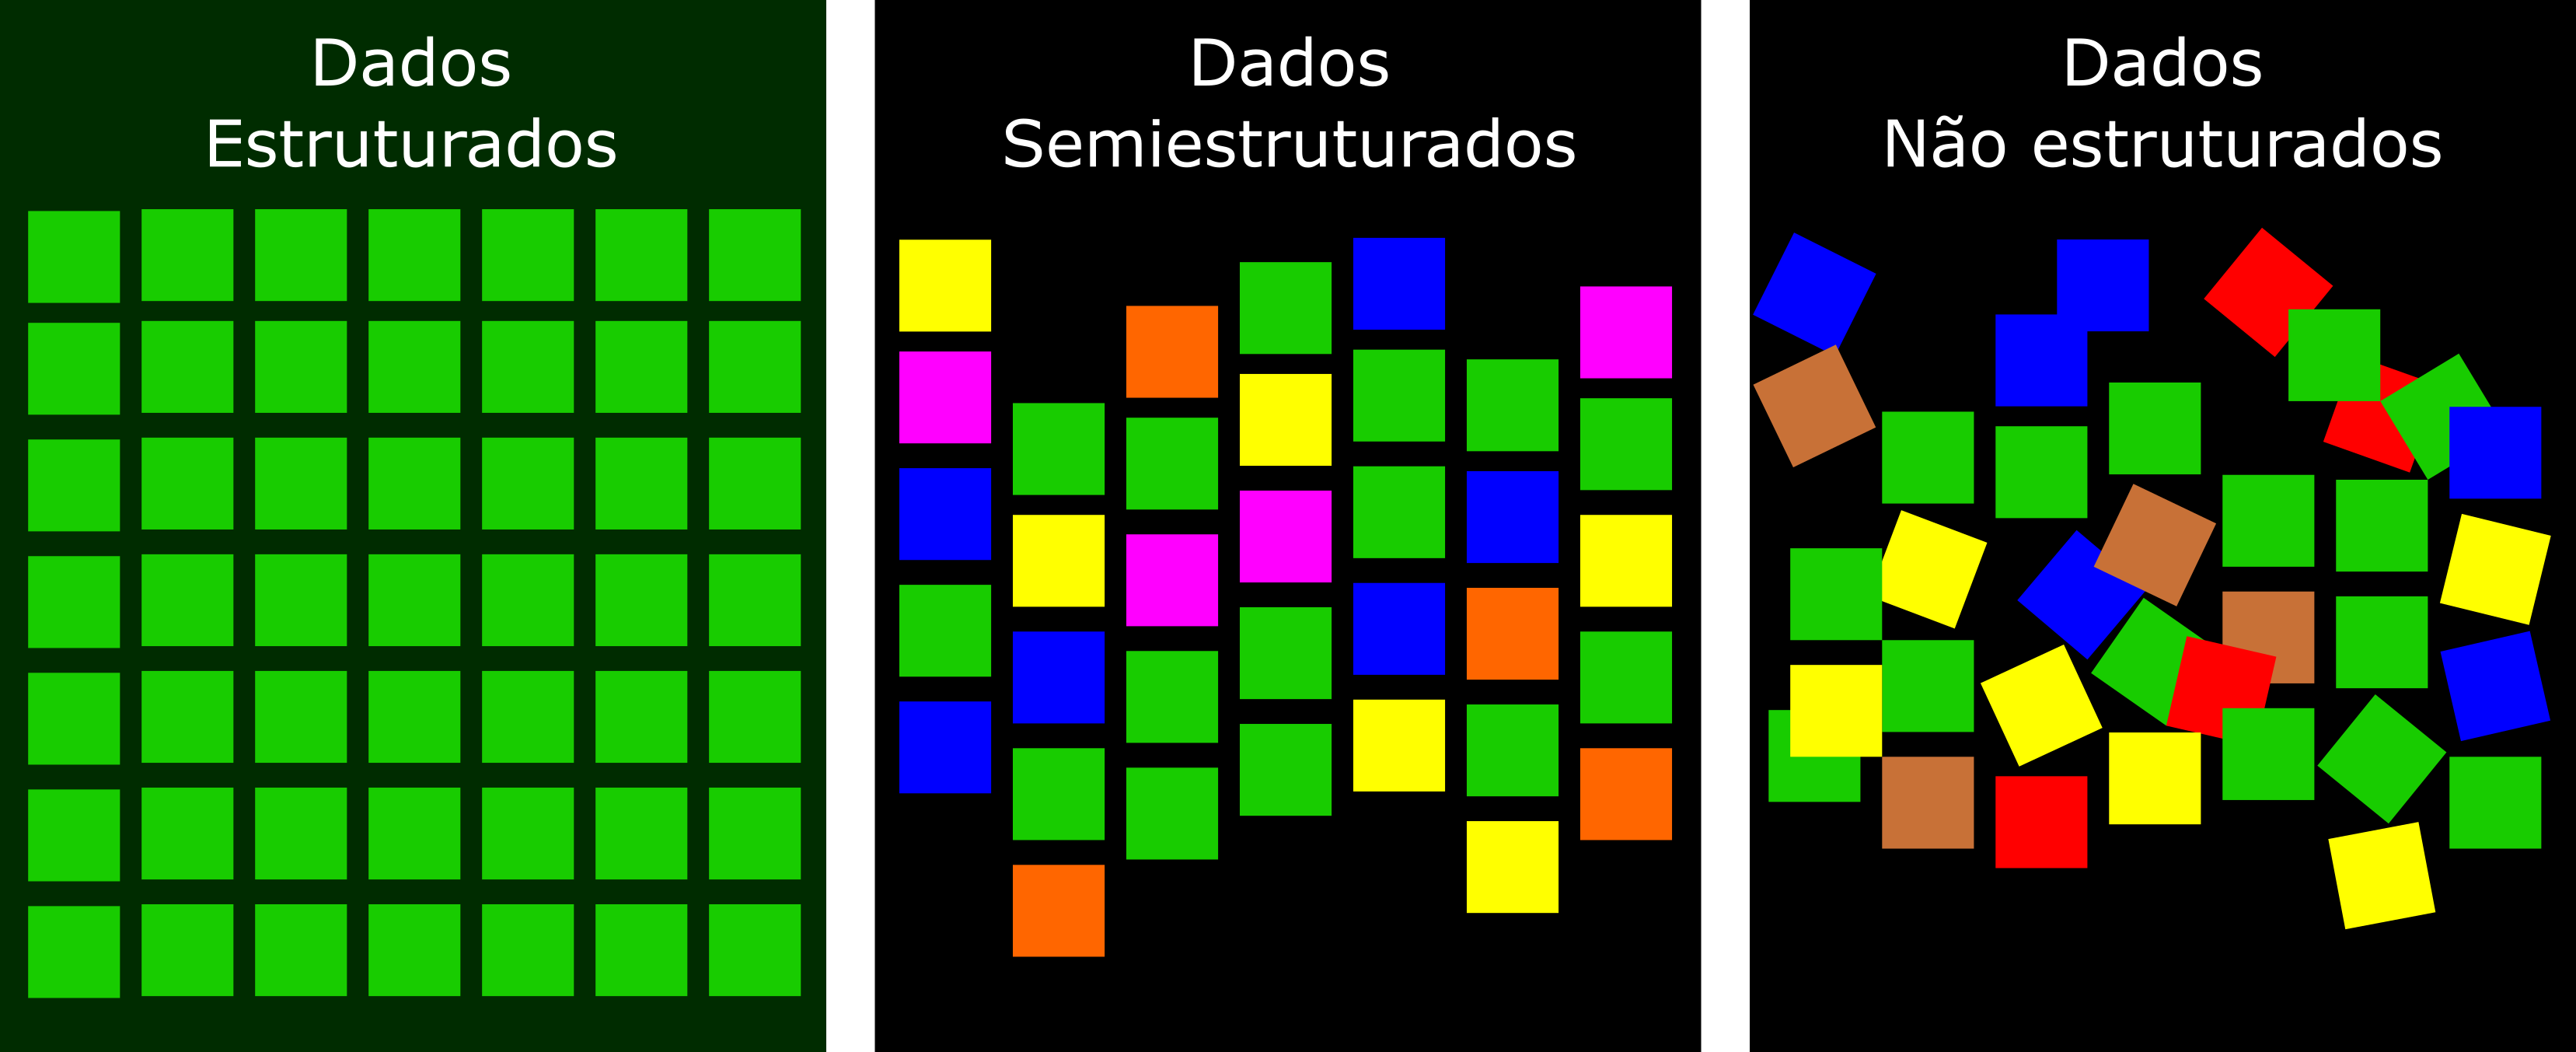
\includegraphics[width=0.9\textwidth]{figuras/dados.png}
		\label{fig:identificador_da_figura}
		\fonte{Autor}
	}
\end{figure}

\observacao{Observação/anotação para conversar com o orientador ou destacar importância.}

Utilize o comando \texttt{$\backslash$tachado\{\}} para tachar um texto. Exemplo: \tachado{comprar} adquirir.

Esse texto é um exemplo para \correcao{destaques de correção} a serem realizadas.

\subsection{Subseção}
\label{subsec:subseçao}
Bla bla bla


% Base Teórica
\chapter{Fundamentação Teórica}
\label{ch:identificador}
	\begin{resumocapitulo}
		Aqui vai um pequeno resumo do capítulo.
	\end{resumocapitulo}

	\section{Visão Geral}
		Neste capítulo devem ser apresentadas as fontes de pesquisa (artigos, teses, dissertações, publicações, etc.). A Fundamentação Teórica é a base para qualquer trabalho acadêmico, de a mostra o que já existe e como isso tem realção com o seu trabalho.

	\section{Conteúdo 1}
	\label{sec:identificao}
        Bla bla

		% Lista numerada
		\begin{enumerate}
			\item Bla
			\item Bla
		\end{enumerate}

		% Lacuna de pesquisa - um bloco para cada lacuna
		\begin{lacuna}
		\label{lacuna:lacuna1}
			Descrever aqui a lacuna de pesquisa. Se tiver mais que uma, criar outro bloco.
		\end{lacuna}
	
		% Pergunta de pesquisa - um bloco para cada pergunta
		\begin{pergunta}
		\label{pergunta:pergunta_1}
			Aqui vai a pergunta de pesquisa 1.
		\end{pergunta}

		\begin{pergunta}
		\label{pergunta:pergunta_2}
			Aqui vai a pergunta de pesquisa 2.
		\end{pergunta}	

% Metodologia
\chapter{Metodologia}
\label{ch:identificador}
	\begin{resumocapitulo}
		Aqui vai um pequeno resumo do capítulo.
	\end{resumocapitulo}

	\section{Visão Geral}
		Descrever uma visão do capítulo. É um resumo mais elaborado que visa posicionar o leitor sobre o que será abordado adiante.

		Aqui deve ser descrito \textbf{passo-a-passo} o que foi feito durante todo o processo até chegar ao resultado final.

	\section{Conteúdo 1}
	\label{sec:identificao}
        Bla bla

		% Lista numerada
		\begin{enumerate}
			\item Bla
			\item Bla
		\end{enumerate}

		% Lacuna de pesquisa - um bloco para cada lacuna
		\begin{lacuna}
		\label{lacuna:lacuna1}
			Descrever aqui a lacuna de pesquisa. Se tiver mais que uma, criar outro bloco.
		\end{lacuna}
	
		% Pergunta de pesquisa - um bloco para cada pergunta
		\begin{pergunta}
		\label{pergunta:pergunta_1}
			Aqui vai a pergunta de pesquisa 1.
		\end{pergunta}

		\begin{pergunta}
		\label{pergunta:pergunta_2}
			Aqui vai a pergunta de pesquisa 2.
		\end{pergunta}	

% Resultado
\chapter{Análise dos Resultados}
\label{ch:resultados}
Descrever as conclusões do trabalho... bla bla bla.

\section{Item 1}
Bla bla bla

% Conclusão
\chapter{Conclusões}
\label{ch:conclusao}
	Descrever as conclusões do trabalho... bla bla bla.


% ##################### Fim dos Capítulos ############################

% Bibliografia (Obrigatório)
\bibliography{refs}

% ##################### Apêndices ############################
\renewcommand{\appendixtitle}{Apêndices}
\begin{appendixenv}
    \section{: Título}
Segundo a ABNT (Associação Brasileira de Normas Técnicas), os apêndices são textos criados "pelo próprio autor" para complementar sua argumentação.
    \subsection*{Descrição}
        \begin{enumerate}
            \item Conteúdo
        \end{enumerate}        
        

\end{appendixenv}

% ##################### Anexos ############################
\renewcommand{\appendixtitle}{Anexos}
\begin{appendixenv}
    \section{: Título}
    Segundo a ABNT (Associação Brasileira de Normas Técnicas), os anexos são documentos criados por terceiros, e usados pelo autor.
    \subsection*{Publicação}
        \begin{enumerate}
            \item DE SOUZA, E. M.; STOROPOLI, J. E. ; ALVES, W. A. L.~\textbf{FERRAMENTA DE EXTRAÇÃO DE DADOS PARA A WEB OF SCIENCE}. \textbf{In}: SETII - Seminário em Tecnologia da Informação Inteligente, 2019, São Paulo. Universidade Nove de Julho.
        \end{enumerate}
\end{appendixenv}

\end{document}